\chapter{User Manual}
\lstset{language=NoBeardAsm}
\section{Overview}
This chapter describes how to use the graphical user interface of the NoBeard virtual machine and serves at the same time as a user manual. With the NoBeard Machine users are able to load and run NoBeard object files with just a view clicks. The integrated debugger of the virtual machine gives them also the possibility to debug these programs by setting breakpoints and stepping through the program in one by one assembler instructions. Another big feature is the data visualization which gives users a whole view of the data memory.
\section{The UI Components}
As shown in figure~\ref{fig:components} the NoBeardMachine contains the following five windows:

\begin{figure}[h] 
	\centering
	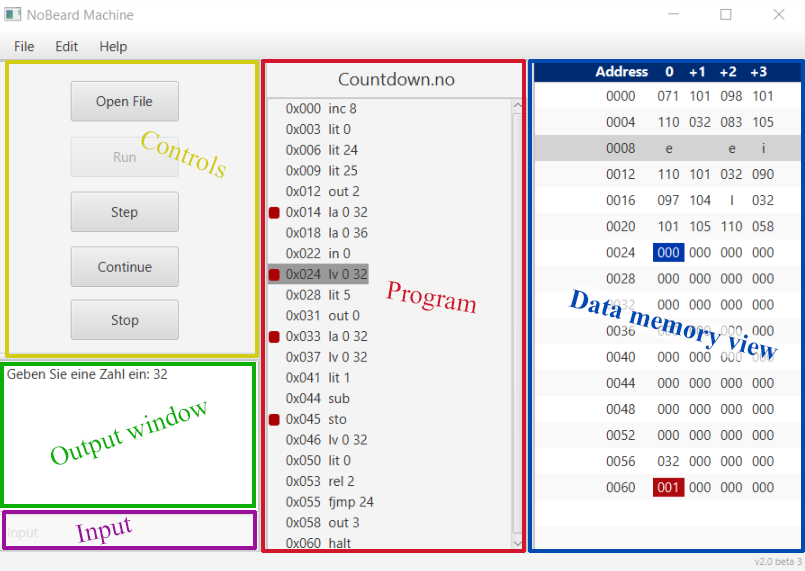
\includegraphics[scale=.87]{images/screenshot-0.png}
	\caption{Components of the NoBeardMachine}
	\label{fig:components}
\end{figure}

\begin{itemize}
\item \textbf{Control Window: }A window with a set of buttons for user interactions.
\item \textbf{Output Window: }A terminal showing outputs of programs and user inputs.
\item \textbf{Program Window: }Shows the actually opened program and its running flow.
\item \textbf{Data Memory Window: }A visualized call stack of a debugged program.
\item \textbf{Input Window: }A single-line field for user inputs.
\end{itemize}

\subsection{Control Window}
This window consists of five buttons that gives the possibility to open, run, stop programs, step between instructions or continue execution from a breakpoints until another one. 
\begin{itemize}
\item \textbf{Open file: }Opens a file chooser dialog where the target object file can be selected.
\item \textbf{Run: }Executes the program from the first instruction. 
\item \textbf{Step: }Allows the user to step one single assembler instruction further in the program flow. This button is only enabled if the machine is in state \lstinline$blocked$.
\item \textbf{Continue: }When the program execution gets interrupted by a breakpoint this button enables users to continue the execution of the program until the next breakpoint or the end of the program. If there is no breakpoints left it continues the process until the end.
\item \textbf{Stop: }Stops the execution and sets the machine into the \lstinline$stopped$ state.
\end{itemize}
\subsection{Output Window}
The output window is a non-editable text area which simulates a terminal. Program outputs that are coming from a NoBeard \lstinline$out$ instruction are shown here. Submitted inputs are also visible here after a successful submit.
\subsection{Program Window}
The program window shows the assembler instructions of the loaded program with the corresponding start address of each instruction. When clicking on the empty area in front of the instruction's address a breakpoint can be set or unset.  
\subsection{Data Memory Window}
A ListView filled with raw data from the data memory. Every line of the ListView contains four byte data with the belonging addresses. The raw data can be converted into different formats like characters or integers to make it better readable to humans. Furthermore the frame pointer and the stack pointer of the currently running frame are highlighted. Each byte can be converted to a character and a whole line can be translated to four characters or to a single four byte integer. Data with blue background color highlights the frame pointer. Red background color stands for the stack pointer.
\subsection{Input Window}
The Input window is a TextField where inputs from users can be handled. It is only enabled when the machine is executing an \lstinline$in$ instruction. To submit an input, the "ENTER" key has to be pressed and then the entered text will be attached to the Output window.

\section{Loading and Running a Program}
After starting the NoBeardMachine, a NoBeard object file has to be loaded by a click on the “Open File” button. Than a file chooser dialog appears where the user can choose the desired file. Afterward the window shows the assembler code and the title of the opened program which is now ready for execution.

The Program window lists the assembler instructions with the belonging operators and addresses in decimal form. By hitting the “Run” button, the machine executes the loaded program. Output results can be seen in the Output window. If the program runs against an input instruction, the machine stops and requests the user for an input which can be done at the Input window. To submit an input, the Enter key has to be pressed. After the user pressed the Enter key the program continues its execution.
\begin{figure}[h] 
	\centering
	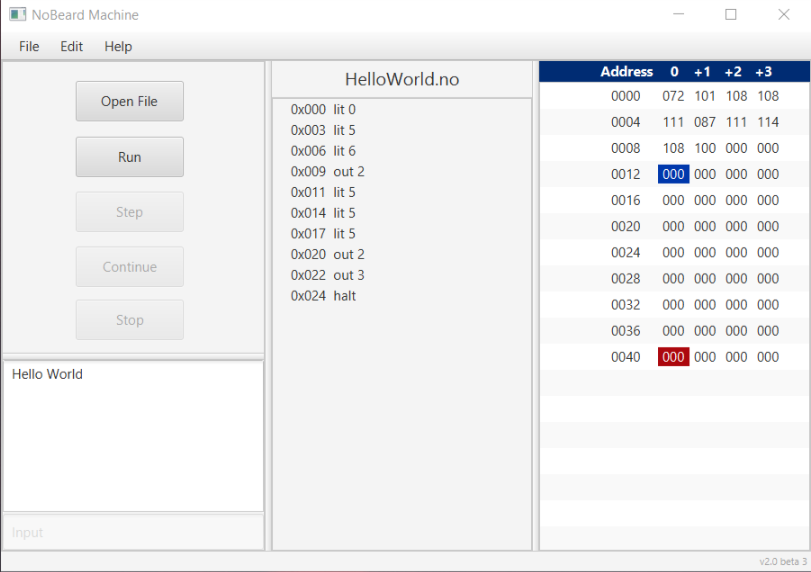
\includegraphics[scale=.85]{images/screenshot-1.png}
	\caption{Executed "Hello World" program}
\end{figure}

\section{Debugging}
To debug a program the user has to set breakpoints which interrupts the program flow and allows the user to inspect the current state of the running program. These breakpoints can be placed by clicking on the address or onto the empty space in front of the address with the instruction where the program flow has to be interrupted. 

After an interruption caused by a breakpoint, the user is able to step one line further or continue execution until to the next breakpoint. Stepping is handled by the “Step” button as shown in figure~\ref{fig:debugging}. By clicking the “Continue” button, the program runs from the current line until the next breakpoint. If there is not any breakpoint left from the current line, it runs until the end of the program. Optionally, the user is able to stop the program during the execution. This could be achieved by clicking the “Stop” button.
\begin{figure}[h] 
	\centering
	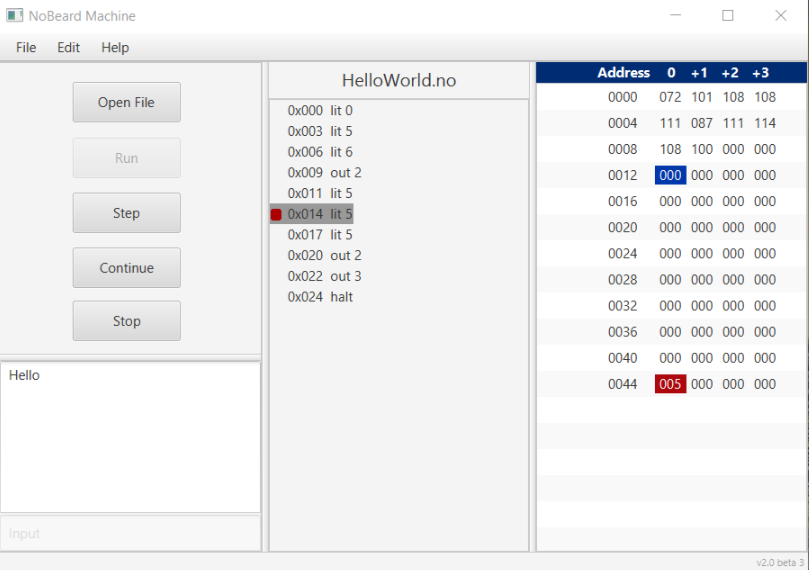
\includegraphics[scale=.85]{images/screenshot-2.png}
	\caption{Debugging the "Hello World" program}
	\label{fig:debugging}
\end{figure}

\section{Data Visualization}
On the right side of the window is the visualisation of the data memory in a ListView form. This window lists data byte-wise from the data memory of the machine. Each line of the ListView has a content of an address given in decimal notation followed by four bytes of raw data. The memory is separated in two parts. The list starts on the top with the string constants followed by stack frames of the currently running functions. While the frame pointer is highlighted with a blue background, the stack pointer is signed with a red background. The user has also the possibility to convert raw data to characters or integers.
With a right click on the selected line of the list, a context menu opens. The context menu includes the following functions which will be described in the sections thereafter:
\begin{itemize}
\item Converting a single byte to character or a whole line to four characters
\item Converting data to integer 
\item Converting a line back to raw data. 
\end{itemize}
\begin{figure}[h] 
	\centering
	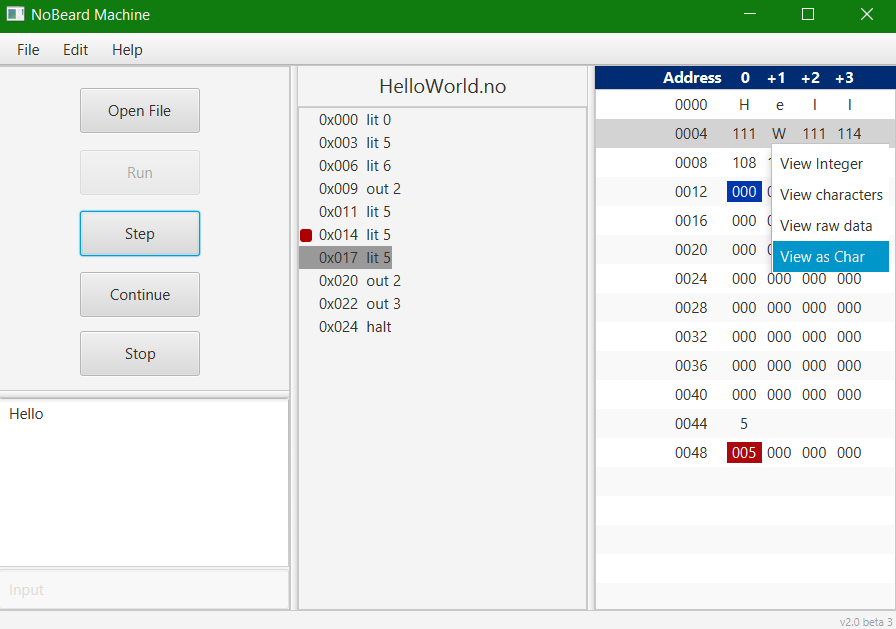
\includegraphics[scale=.80]{images/screenshot-3.png}
	\caption{Converting data to a character}
	\label{fig:convertToChar}
\end{figure}
\subsection{Converting Data to Character}
To view a character of a one-byte data as shown in figure~\ref{fig:convertToChar}, the following steps have to be done:
\begin{enumerate}
\item Select the line where the one-byte value is located 
\item Right click on the value to be converted
\item Click on "View as Char" 
\end{enumerate}
Now the value at the given address is translated to an alphanumeric character. 
The conversion of an entire row of data to characters is done in the same way except that the user has to click "View characters" instead of "View as Char"
\subsection{Converting Data to Integer}
The translation of an integer takes four bytes that means, it takes four data cells from the desired start address and translates them to a single integer.  
\begin{figure}[h] 
	\centering
	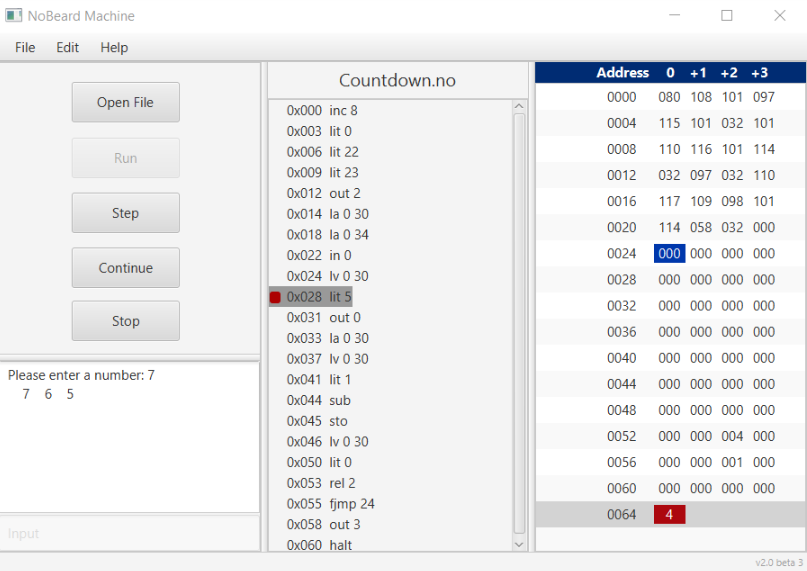
\includegraphics[scale=.90]{images/screenshot-4.png}
	\caption{Converting four-byte data to a single integer}
	\label{fig:convertToInt}
\end{figure}
\begin{enumerate}
\item Select the data cell with the start address of the integer
\item Right click on the cell
\item Click on "View Integer"
\end{enumerate}
After a successful conversion, the four data cells are being replaced by a single integer. Figure~\ref{fig:convertToInt} shows an example of the translated integers. The first one is at address 54 which is not aligned in one row and the second one is on the same place as the stack pointer, precisely at the address 64. 

\subsection{Multiple Conversion}
To facilitate the conversion from raw data to alphanumeric characters a multi selection function is available for the list of the data memory.
To convert multiple data rows, the user has to hold the "Ctrl" key and select the specified rows with a left mouse click. Chosen lines will get highlighted with a light grey background color. As figure~\ref{fig:multipleConversion} shows, the selected rows with grey background are successfully concerted to some characters.
\begin{figure}[h] 
	\centering
	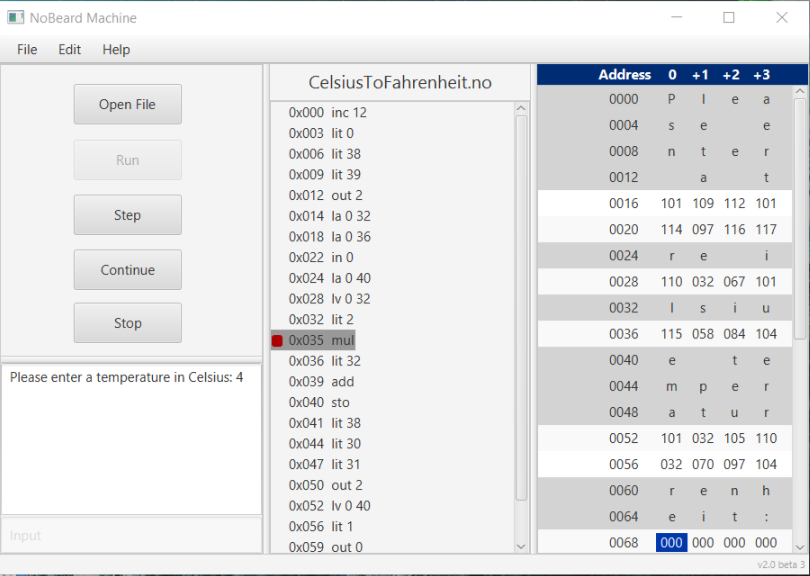
\includegraphics[scale=.85]{images/screenshot-5.png}
	\caption{Multiple conversion of data}
	\label{fig:multipleConversion}
\end{figure}
